\documentclass[UTF8]{article}
\pagestyle{plain}
\usepackage{graphicx}
\usepackage{ctex}
\usepackage{float}
\title{经济学科普: \\ 1.理性预期革命}
\author{白纸}
\date{\today}
\begin{document}
\maketitle

\section{参考内容}
    保罗·沃尔克,《坚定不移:稳健的货币与好的政府》\par
    威廉森,《宏观经济学》\par
    李斌、伍戈,《信用创造、货币供求与经济结构》\par
    徐高,《宏观经济学二十五讲:中国视角》

\section{变革}
    大家熟知的学科的变革有哪些呢?\par
    物理方面,经典力学的建立、相对论的提出、量子力学体系的建立,这些都是物理上的变革。
    数学方面,牛顿和莱布尼茨创立微积分、康托尔创立集合论、勒贝格提出勒贝格积分等等。\par
    这些学科的变革有一个共同特点,就是:虽然提出了新的概念,但是对过去的内容没有全面的否定,
    过去的内容在某些情形下仍然适用。比如经典力学仍然在机械、土木、航空等众多领域发挥重大作用;
    大家在本科仍然学习黎曼积分,工科很少会接触到勒贝格积分。\par
    那么经济学在这些年有没有重大的变革?经济学作为社会科学,变革之后的新概念对之前的内容有多大的冲击?\par
    这篇文章会慢慢给大家讲述。

\section{菲利普斯曲线的消失}
    菲利普斯曲线,是20世纪50年代被发现的\textbf{通货膨胀率与失业率之间的负相关关系}。
    这一现象最早由新西兰经济学家威廉·菲利普斯在1958年提出。\par
    在他发表的《1861-1957年英国失业和货币工资变动率之间的关系》一文中,
    菲利普斯提出通货膨胀率与失业率之间存在负相关关系。这种关系在
    美国数据中也被发现,后来大家就把这种通货膨胀率和失业率之间的负相关关系称作菲利普斯曲线。\par
    (注:中国的失业率数据存在质量问题等原因,数值缺乏足够波动性,以此估计的菲利普斯曲线不够理想,
    现实中采用失业率构建中国的菲利普斯曲线的实证研究不多见。)\par
    
    \begin{figure}[H]
        \centering
        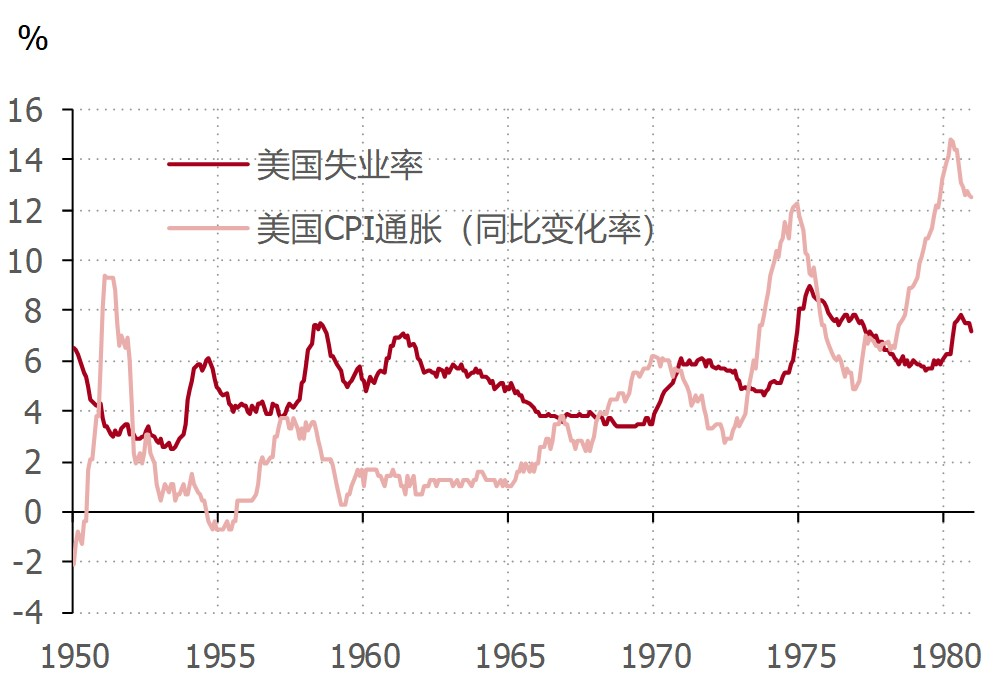
\includegraphics[width=9.9cm,height=6.8cm]{美国失业率与通胀走势.jpg}
        \caption{美国失业率与通胀走势}
    \end{figure} 
    图1中,可以看出在1954-1966年,通货膨胀率与失业率之间明显的负相关关系。因为菲利普斯曲线是
    如此的明显,同时在多个国家都能发现这种规律,所以它很快就被视为宏观经济的基本事实之一,被写入
    了当时标准的宏观经济模型,成立凯恩斯宏观经济学的一块基石。\par
    对于政府来说,失业率的下降可以让社会更稳定。因此,如果付出一点通货膨胀升高的代价,就能让失业率下降,
    这显然是比较好的政策,政府也能获得更高的支持率。\par
    在20世纪70年代石油冲击之后,美国开始有意识地通过推高通货膨胀来压低失业率。\par
    然而!!!\par
    当政府开始利用菲利普斯曲线来调控经济时,高通胀并没有带来更低的失业率,反而
    造成了\textbf{滞胀}(高通货膨胀和高失业率)。\par
    \begin{figure}[H]
        \centering
        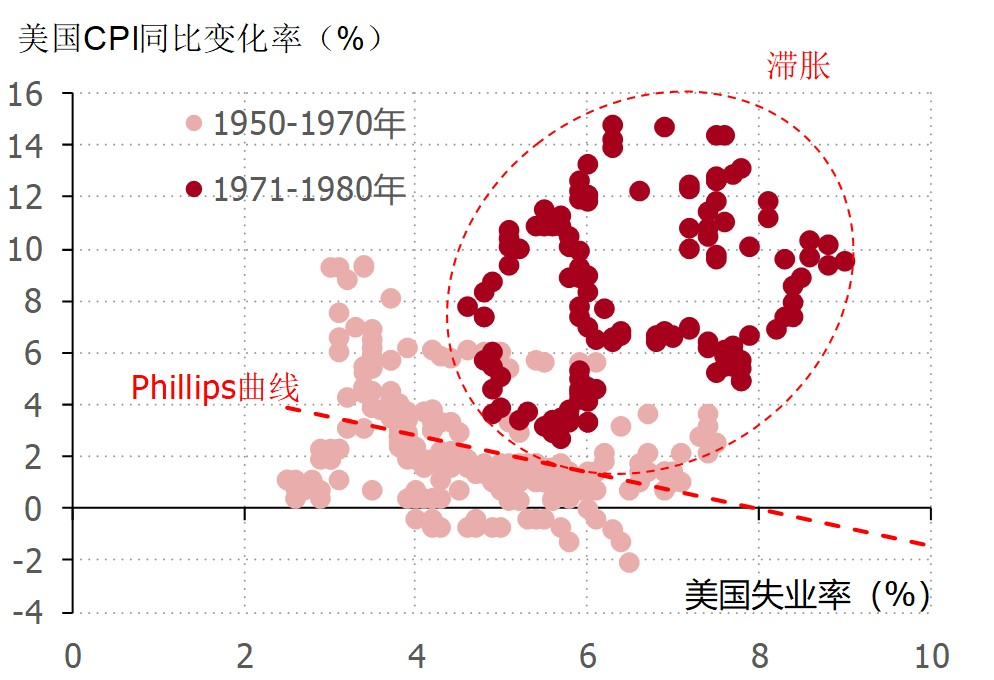
\includegraphics[width=9.9cm,height=6.8cm]{菲利普斯曲线.jpg}
        \caption{美国菲利普斯曲线的消失}
    \end{figure}
    图2中,可以看出1950-1970年,CPI同比与美国失业率呈现明显斜线。然而在1971-1980年,呈现了
    圆形(为什么会是圆形,之后的文章会讲到)。\par
    滞胀的出现对当时的经济学理论(基于凯恩斯理论)来说,可谓是巨大的冲击。这种来自现实的冲击
    促进了经济学理论的变革与发展。

\section{菲利普斯曲线消失的影响}
    1975年,罗伯特·卢卡斯发表了《经济计量政策评估:一项评论》(Econometric Policy Evaluation: A Critique),这篇文章
    提到:用观察到的历史数据之间的数量关系来评价经济政策调整的效果是无效的。如果历史数据用的是高度加总的宏观数据,则更是
    如此。卢卡斯批判作为学者对经济研究方法的开端,掀起了一场宏观经济学的革命:\textbf{理性预期革命}。自此,经济学的研究方法发生了
    巨大的改变。\par
    货币政策有点类似。如果只看到货币总量$M_{2}$,没有看到货币传导路径,对货币的理解就会出现偏差。\par
    在理性预期革命之前,经济学家认为宏观经济就像是一台机器,只要弄清楚各个宏观经济变量(构件)之间的关系,找到各个变量(
    各个构件)之间的规律,建立数学模型,就可以描述整个宏观经济(机器)。\par
    在理性预期革命之后,经济学家意识到:宏观经济变量之间的数量关系建立在人的行为之上,受到人的预期的影响。预期改变,人的行为
    就会改变,之前的经济变量之间的数量关系不再稳定。\par
    比如消费:\textbf{当前的消费是基于对未来的预期}  。如果A所在的公司发生了严重的危机,A当月的工资没有改变,但是A对未来
    收入的预期下降,A会降低当月的消费。计算数学专业的硕士B,今年25岁,之前在字节跳动,离职后在家休息了20天,但是B
    不会大幅降低自己的消费,因为B对未来的收入仍有较好预期。当前收入与当前消费之间不存在稳定的数量关系,凯恩斯在
    《就业、利息和货币通论》中描述的消费函数(经济中的总消费是总产出的函数,$C = c_{0} + c_{1}Y$,C:总消费;Y:总产出;
    $c_{0}$,$c_{1}$:两个参数)并不存在。

\section{菲利普斯曲线消失的原因}
    经济学家发现了一些宏观经济变量间的规律,政府试图用这种规律指导政策,却没想到规律本身受到政府行为的影响。\par
    在1950年代,政府没有刻意制造通胀,群众观察到轻微的通胀,会认为经济形势很好,大家都有动力去工作,失业率就比较低
    (有点像14、15年的互联网,大家普遍认为去互联网工作,努力和奋斗是知乎上的关键词汇)。\par
    当政府有意识地通过推升通货膨胀来压低失业率,群众就意识到了通货膨胀是政府多印的钞票,不代表经济形势变好,也就不会
    因为通货膨胀上升而更多地工作。\par
    因此,更高的通货膨胀不会压低失业率,反而带来了高通货膨胀和高失业率的滞胀,菲利普斯曲线消失了。

\section{理性预期革命}
    自理性预期革命之后,宏观经济学模型都开始以微观个体的理性出发,以各个相关主题的最优化问题为宏观建模的基础,
    经济学家看待世界的方式发生了改变。
    \textbf{政府在思考宏观政策时,也会充分预估民间对宏观政策的最优反应,在设计政策时就会考虑到这些反应}。\par
    PS:目前国内的宏观经济学教材主要是:初级宏观经济学、中级宏观经济学、高级宏观经济学。在中级和高级之间,有非常大的
    区别:中级的教材中,有不少基于宏观经济总量的模型,而这些模型可能是不稳固的,这种机械看待宏观经济学发展的方式
    也是错误的;高级的教材中,都是从微观个体优化出发建立的宏观模型。

\section{下一篇的内容}
    下一篇的内容会简单介绍供给与需求曲线、萨伊定律和马尔萨斯需求,根据供求曲线和宏观数据,科普一下什么
    很多经济学理论在美国适用,在中国不适用。

\section{附录}
    那么如果按照现在宏观经济学的思考方式,该如何思考问题呢?以拉姆齐模型为例,
    这里介绍一下如何从微观个体的理性出发,以各个相关主题的最优化问题为基础,建立宏观模型。
    \subsection{仅居民积累资本}
        为了简化模型,这里做了一些假设:
        \begin{itemize}
            \item [1)]
                时间只有2期,第二期期末就是世界末日。居民会在第2期把所有资源消耗光,只在第1期进行储蓄
            \item [2)]
                假设资本不会折旧
        \end{itemize}
        
        \begin{figure}[H]
            \centering
            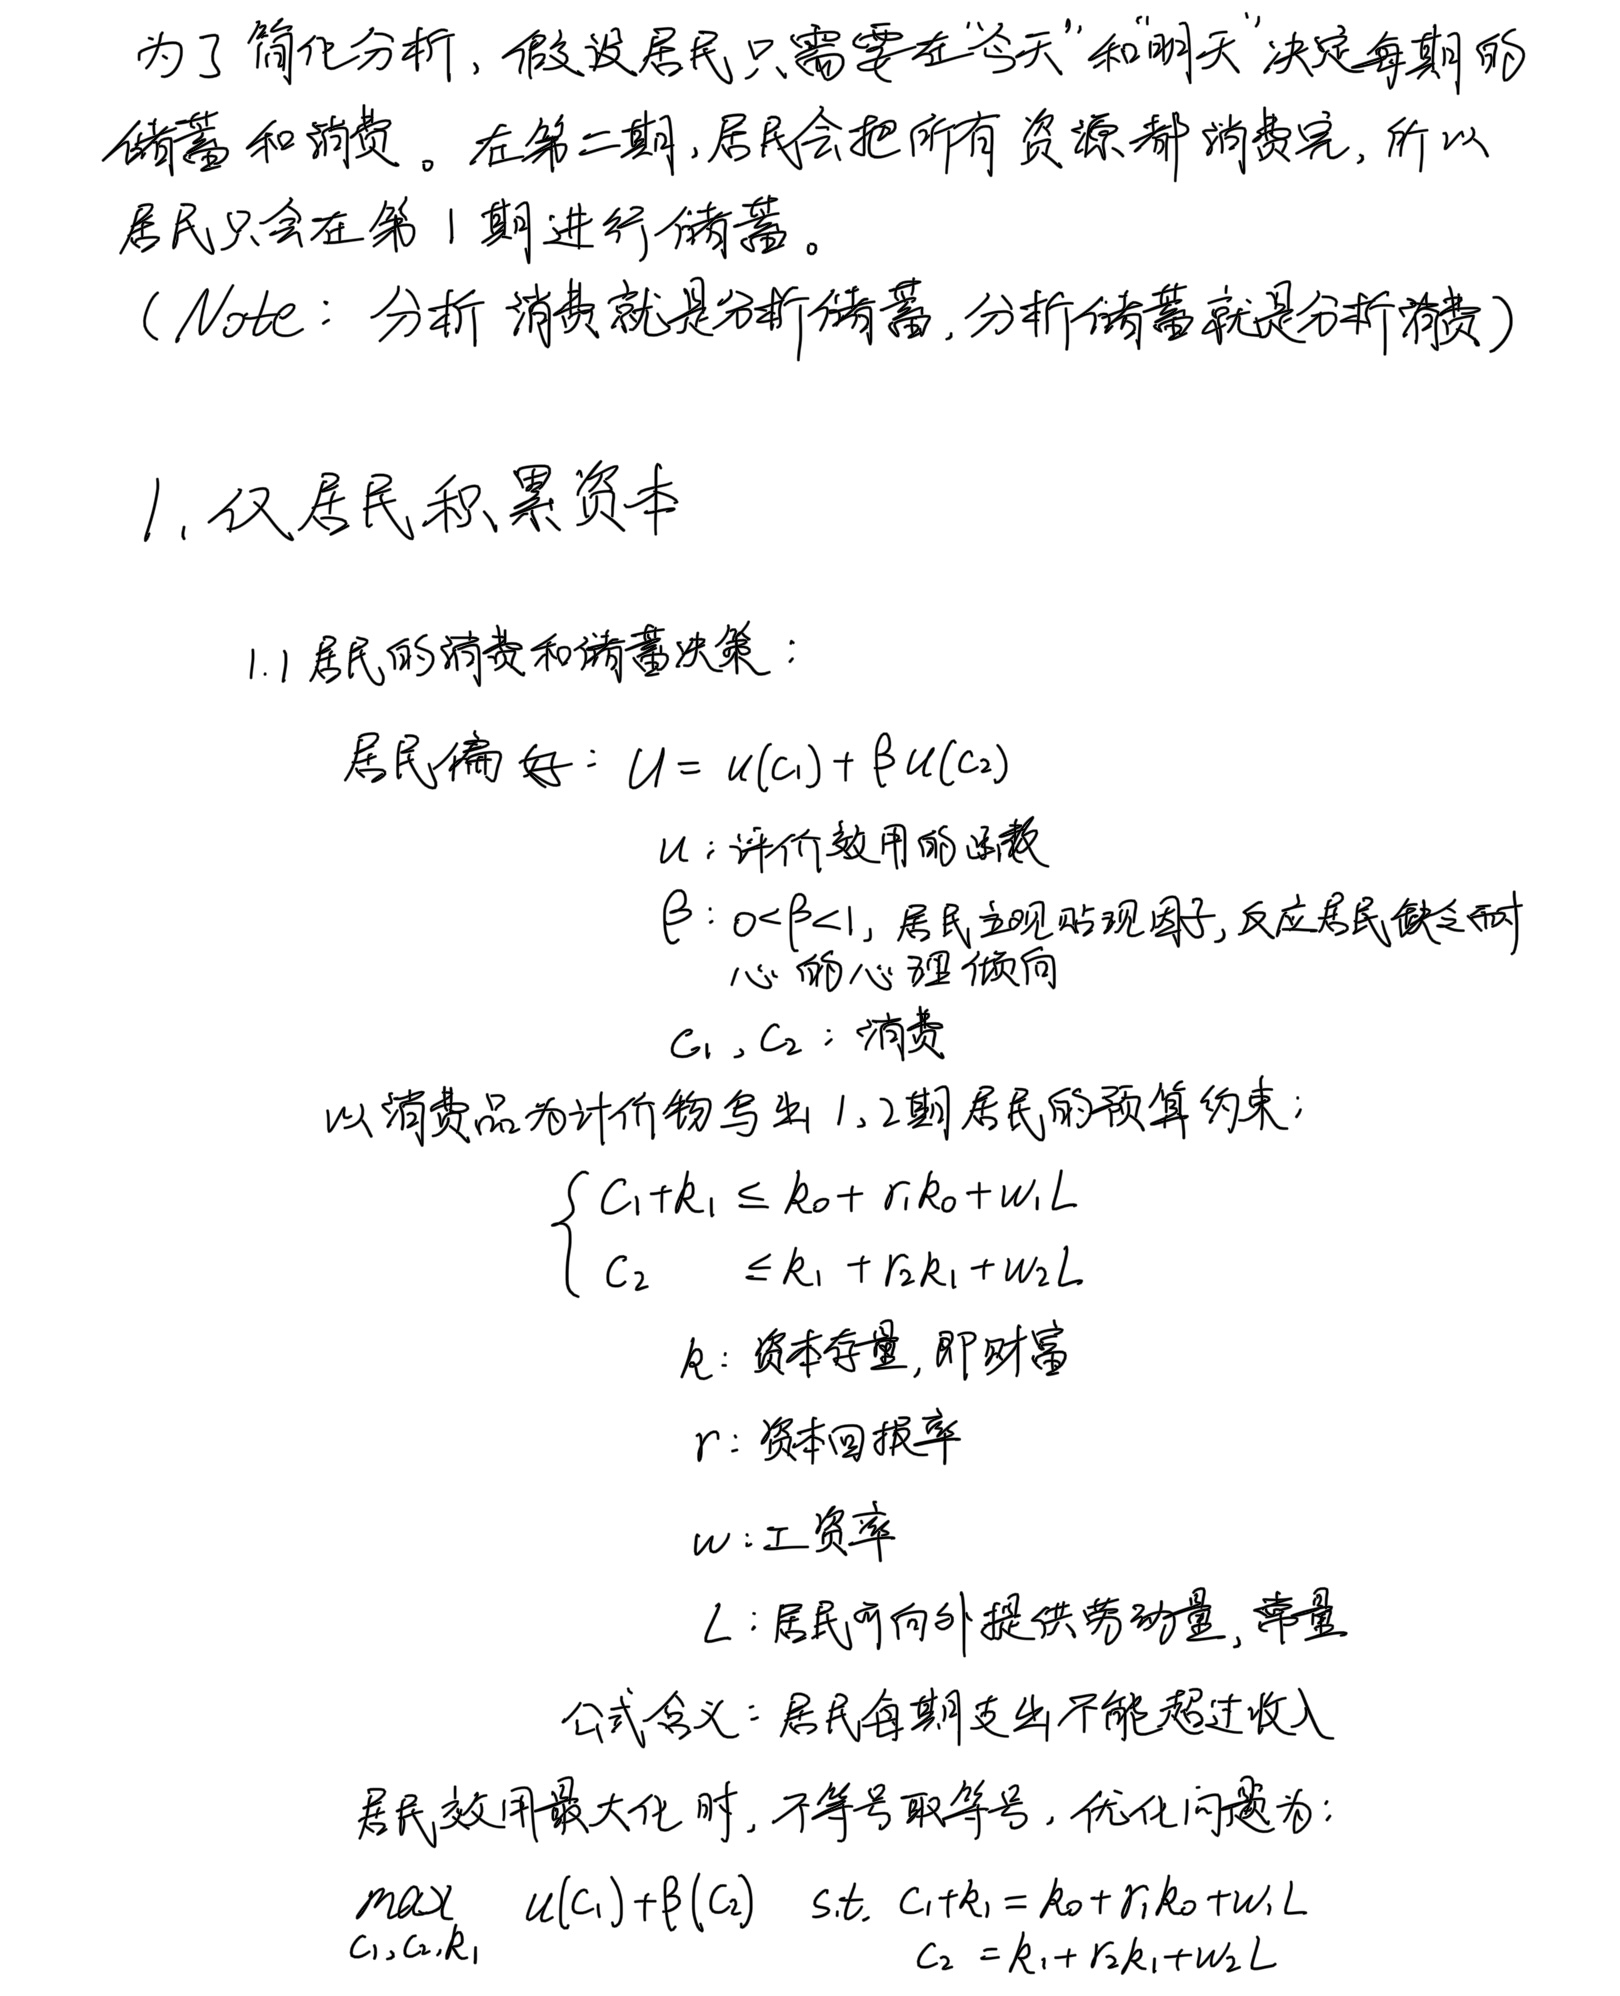
\includegraphics[width = 1 \textwidth]{仅居民积累资本1.png}
            \caption{居民的模型}
        \end{figure}
        \begin{figure}[H]
            \centering
            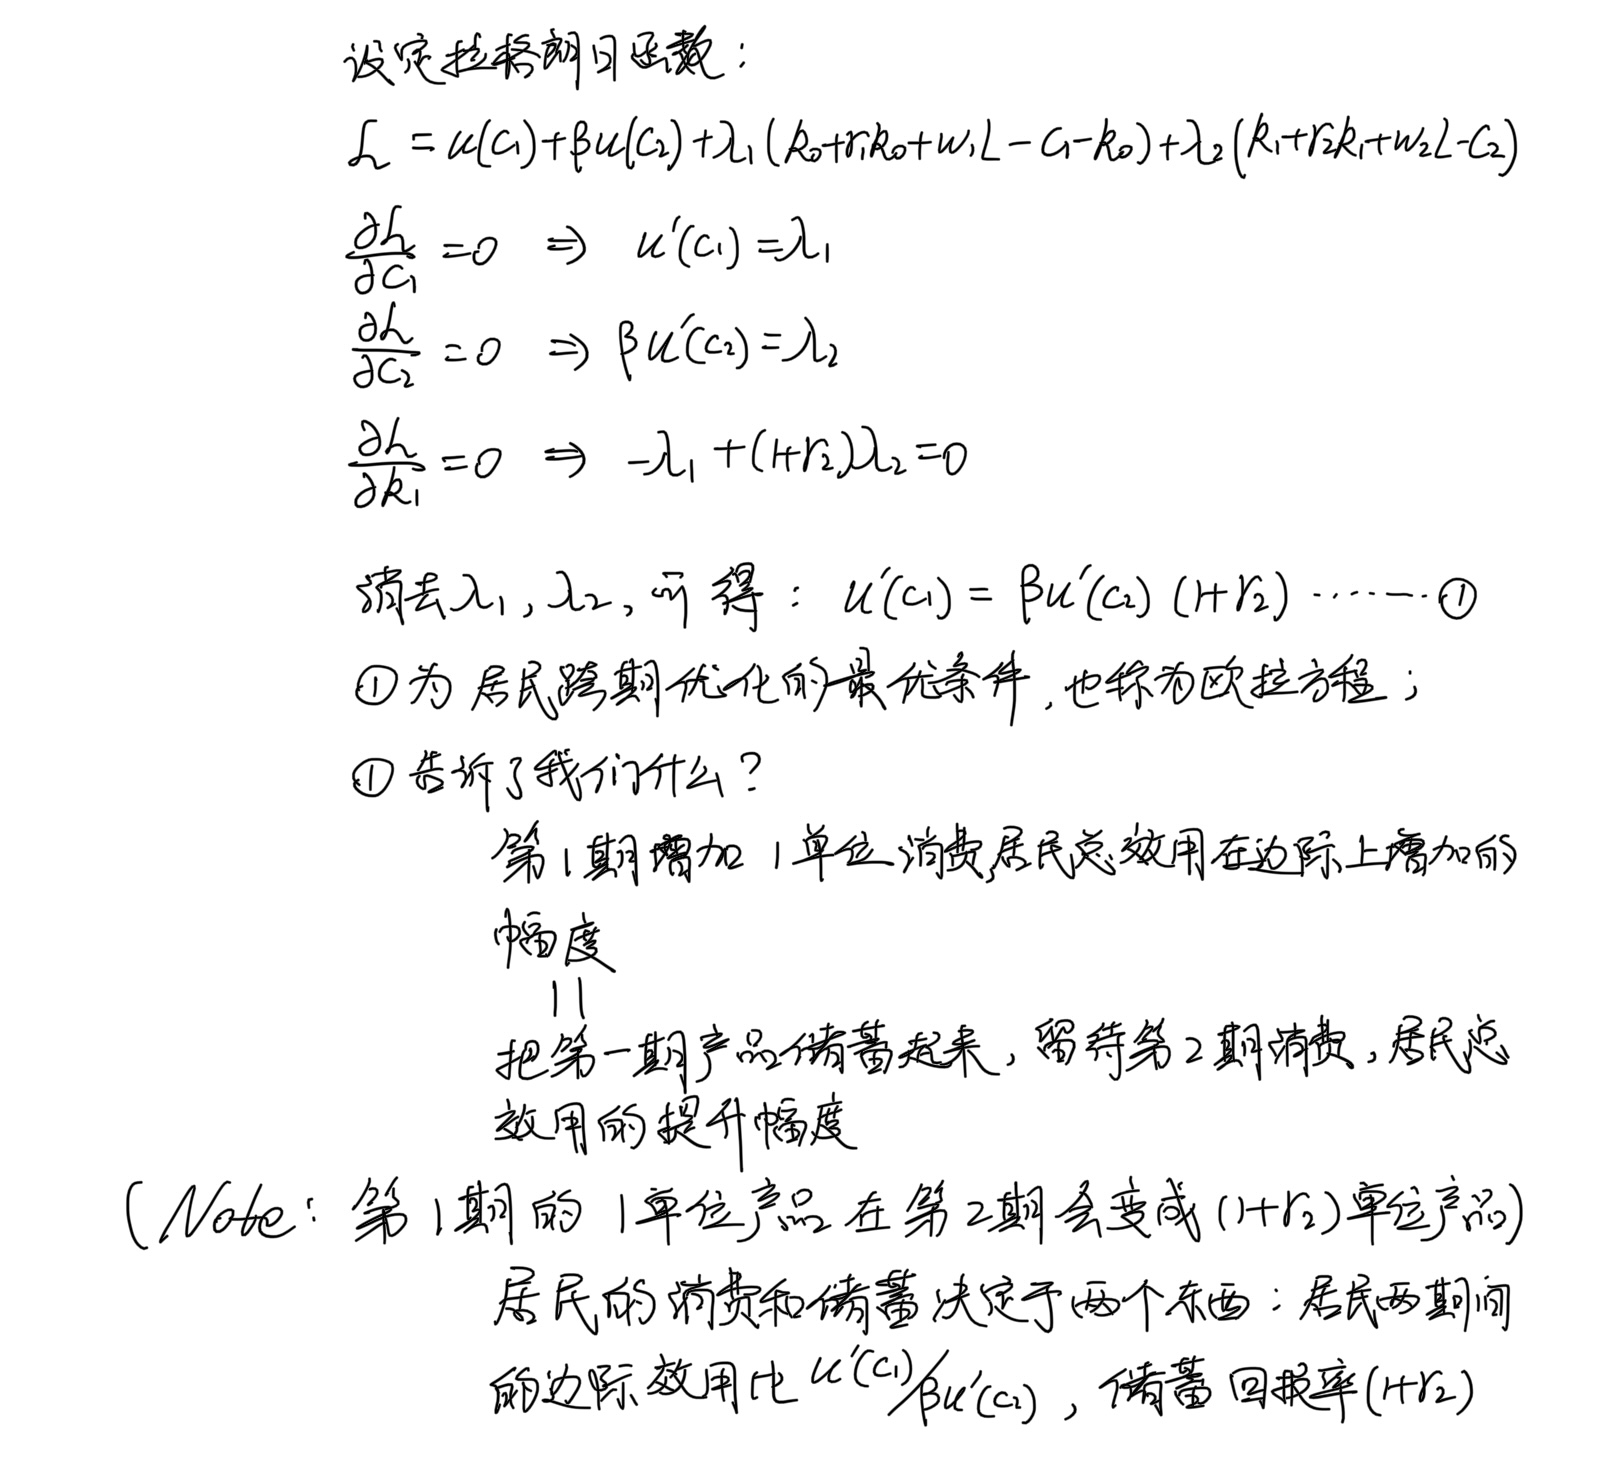
\includegraphics[width = 1 \textwidth]{仅居民积累资本2.png}
            \caption{居民最优化}
        \end{figure}
        \begin{figure}[H]
            \centering
            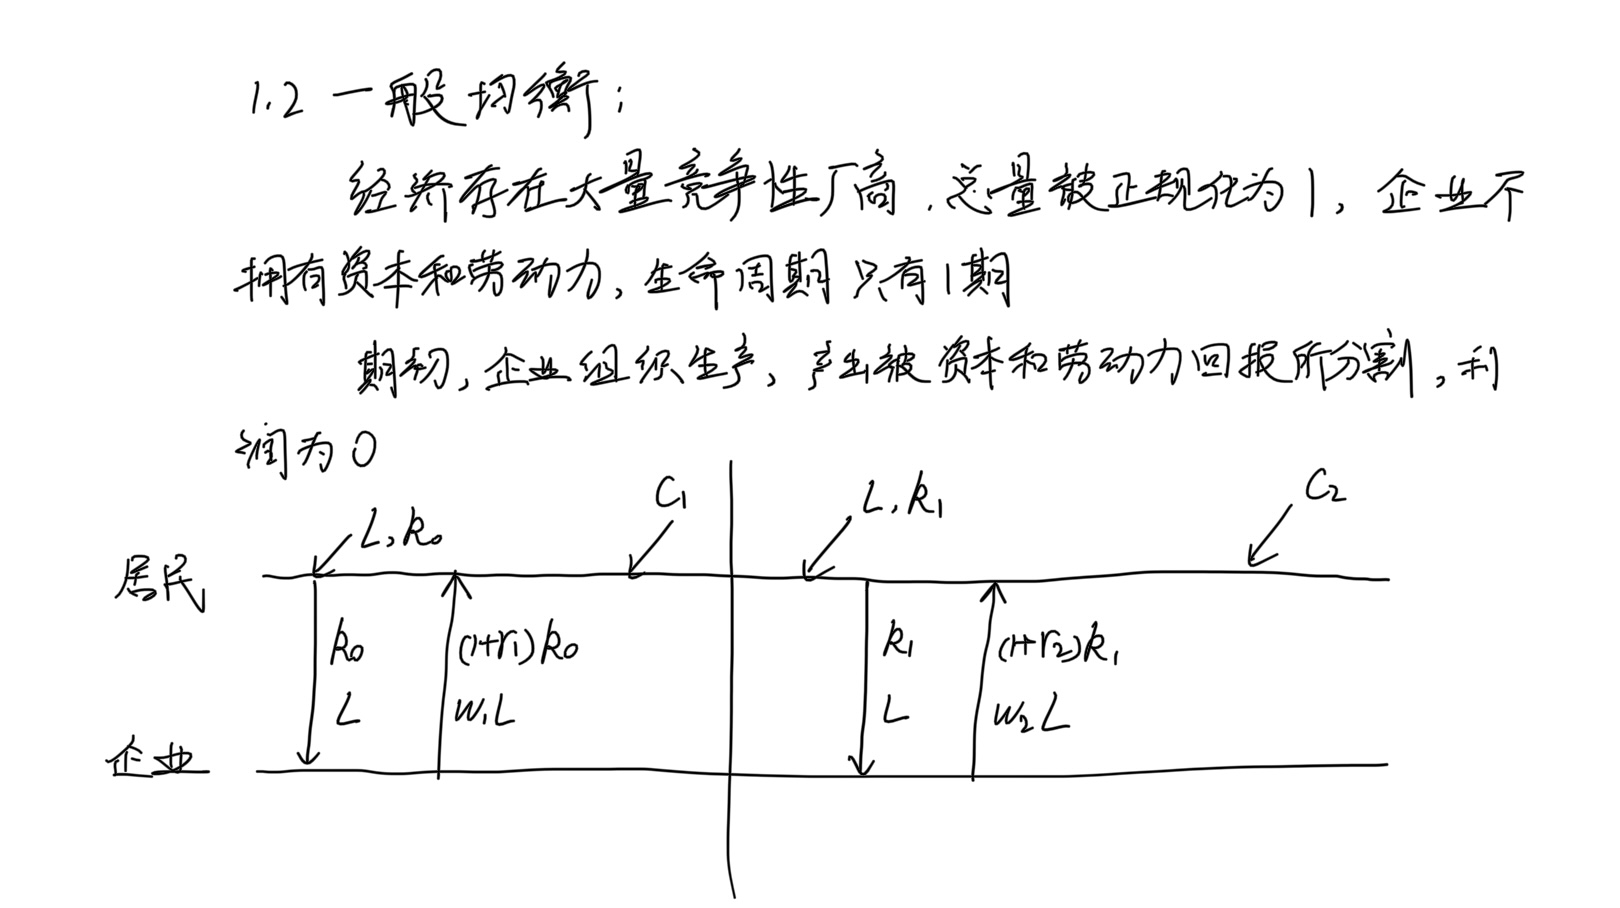
\includegraphics[width = 1 \textwidth]{仅居民积累资本3.png}
            \caption{时序图}
        \end{figure}
        \begin{figure}[H]
            \centering
            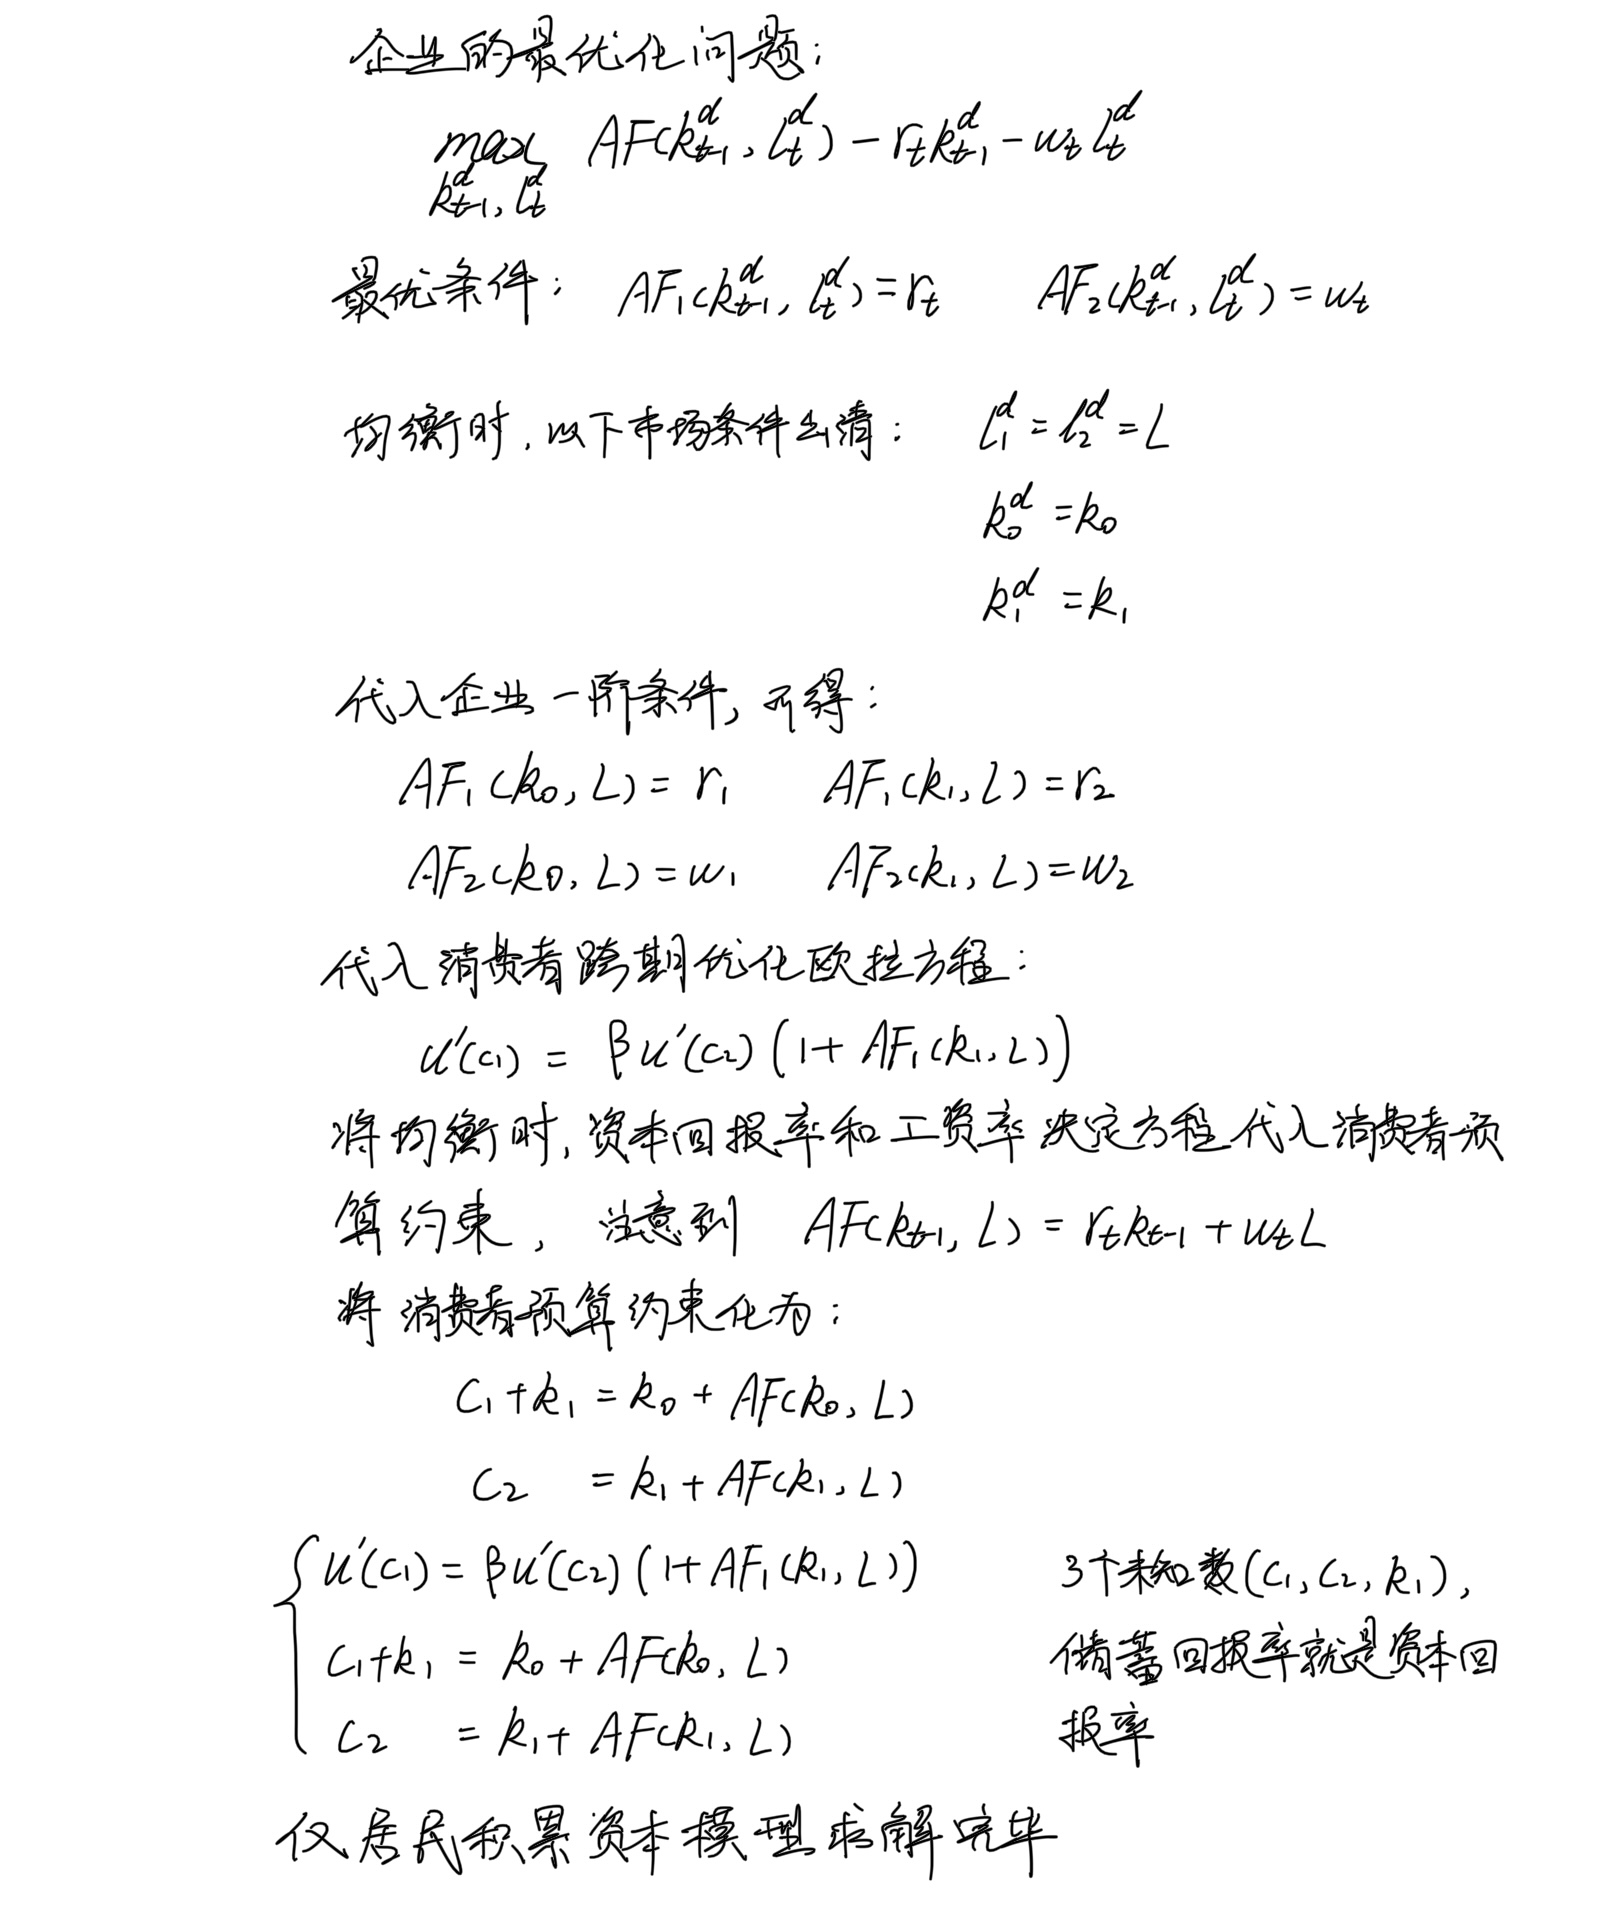
\includegraphics[width = 1 \textwidth]{仅居民积累资本4.png}
            \caption{求解模型}
        \end{figure}

\end{document}